\chapter{Introduction}

% \section{Main Idea}
We are living in the digital era where a mobile phone is everybody's best friend. The internet is all around us, and it almost feels like a commodity. We consider it a fundamental human right, like water. We are used to be online every day from the moment we open our eyes until the moment we shut them again at night. We are obsessed with immediate access to information. That is why mobile applications are so significant these days. They provide a quick way of finding the data that we are interested in. We live quickly and we want to simplify and speed up some tasks. This is where mobile programs come in handy. Opening a web browser, entering an address and logging in takes lots of time compared to a single click on an app icon.

Not so long ago mobile phones allowed only for calls and messages. After some time simple applications started to appear. Most of them were mobile games that you could download on your computer and transfer to your device. You could also download them using, then very slow, Internet connection and WAP protocol. Currently, there are stores where users can search for apps by name, type or functionalities. It is very comfortable because customers can find everything that they want in one place. It is also convenient for developers because they get access to bigger audience when publishing their program on such a platform.

On the other hand, we could use our computers for all tasks. The problem is that they are massive and heavy in comparison to phones. We carry the latter with us everywhere. They allow us to connect to the Internet, use built-in GPS, gyroscope, Bluetooth, cameras, and more. To use computers, also laptops, we have to sit down, turn them on, sometimes log in, only then we can order some things or browse the Internet. That is why there is a need for mobile applications. They allow us to pay phone bills, order clothes, play games, and chat with friends whenever we go. It does not matter if we are traveling in a metro or lying on a couch in a living room.

% TODO - write why I chose the topic
% TODO - write about iOS and Android, normally separate applications for both
% TODO - can I write that my university system (JSOS) works terrible on mobiles and this is what inspired me to create the app? 

\section{Objectives and Scope of Thesis}

%  TODO - add more details

The main objective of this thesis is to create a mobile application for both iOS and Android, which will allow users to log in and get access to data published in a student service system. It will store some of the information in a local SQLite database to let users access them offline. Thanks to it, students will be able to see the details when the student services system is down, or they have limited access to the Internet.

First, users will have to choose their university and log in using credentials for their educational institution system. The mobile application will allow them to access:
\begin{itemize}
    \item news feed for a university or faculty;
    \item profile details;
    \item calendar with class details;
    \item list of grades for every semester;
    \item messages and their details;
    \item list of payments.
\end{itemize}

Besides the mobile application, the project requires a server that will act as a service transforming data between two schema-incompatible systems. The app will send a data request to the server using JSON format. This request will be processed there, mapped to a schema of a selected student services system. After it has been mapped, it will be sent to the system requesting data. The last step is to transform the received information and return it to the mobile application in an expected format. The mapping files for universities will be created using the YAML language. This structure will allow the system to be easily expanded with new universities.

\section{Review of Existing Solutions}

Two similar solutions exist in Poland. Both of them are represented in Figure~\ref{fig:similiar-solutions}. One was explicitly created for the University of Warsaw. We draw inspiration from it to include some functionalities like news feed and mailbox in our project. Unlike the first app, the second one can show data for more than one university. Users have to choose what university they attend, and then they can see their calendar, grades, and some other data from the chosen university system. This is what we wanted to achieve while designing our application. Most of our attention went to creating a simple and extensible API. The program represented in the document was designed to provide better user experience than the second solution described here, and it is supposed to be easily expendable by YAML files, new widgets, and views.

% TODO - ask if I can use these graphics and how to link them

\begin{figure}[htb]
    \centering
    \begin{tabular}{@{}ll@{}}
        a) & b) \\
        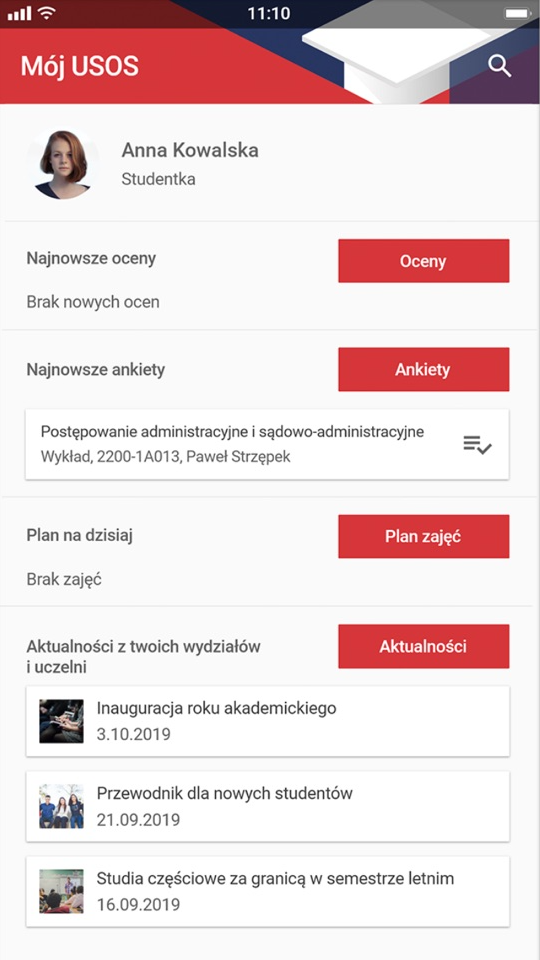
\includegraphics[width=0.425\textwidth]{fig01/mobilny-usos.png} &
        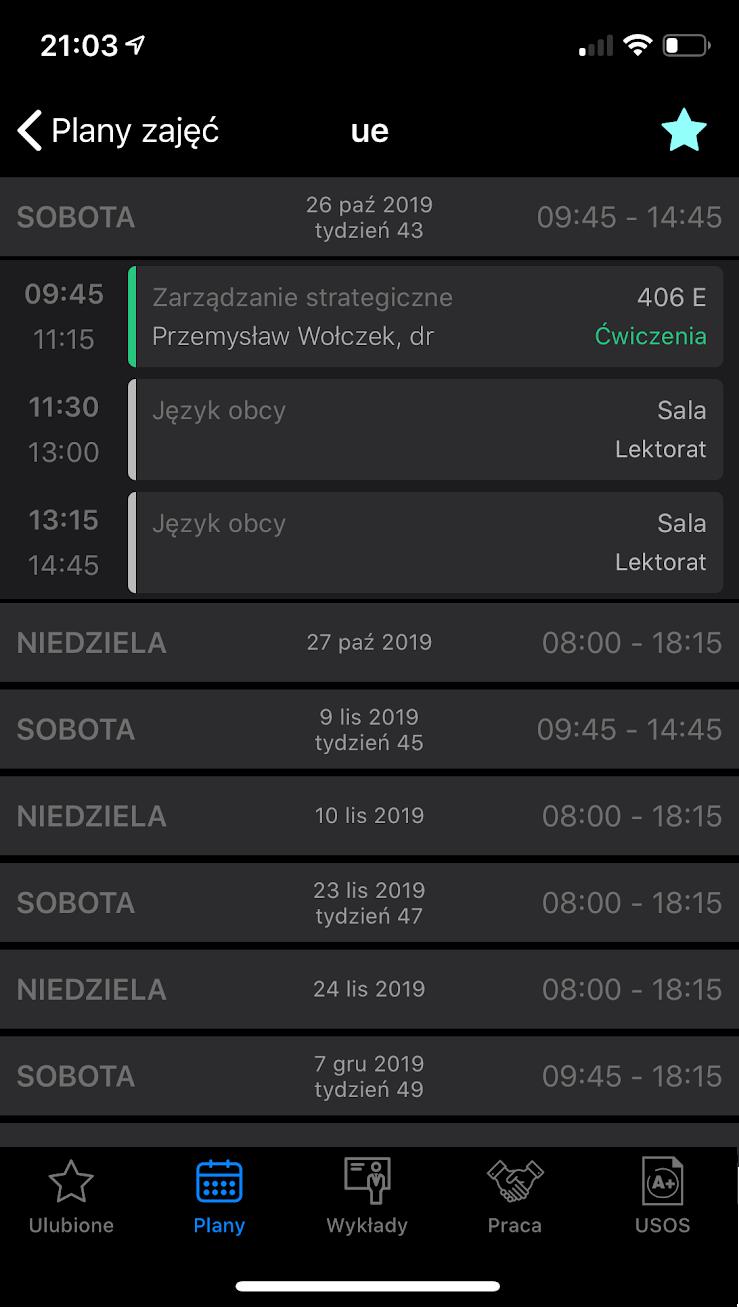
\includegraphics[width=0.425\textwidth]{fig01/kiedy-wyklad.png} \\
    \end{tabular}
    \caption{Similar solutions existing in Poland: a) Mobilny USOS UW, b) Kiedy wykład} \label{fig:similiar-solutions}
\end{figure}

\section{Thesis Structure}

% TODO - describe the structure
